% TeX encoding = utf8
% TeX spellcheck = pl_PL 

\chapter{Wykorzystany sprzęt i~narzędzia}
\label{ch:sprzęt_i_narzędzia}

	\section{Robot IRp-6}
	\label{s:robot_irp6}
	Laboratorium 012 Wydziału Elektroniki i~Technik Informacyjnych wyposażone jest w~dwa roboty typu IRp-6. Bazują one na manipulatorach IRb-6, o pięciu stopniach swobody\cite{merapiap}, które odznaczyły się w~historii robotyki jako pierwsze elektryczne roboty przemysłowe sterowane za pomocą mikroprocesorów\cite{ABB}. Oba manipulatory Politechniki rozbudowano o~kiście pozwalające na obrót nadgarstka, a~jeden z~nich dodatkowo może poruszać się wzdłuż toru jezdnego. Ostatecznie manipulatory \textit{Postument} i~\textit{Track} posiadają kolejno sześć oraz siedem stopni swobody\cite{IRPOS}. Zastosowanie czujników położenia stawów pozwala na precyzyjny ruch, szczególnie ważny przy zadaniach przemysłowych i~badawczych. 
	\section{Robot Velma}
	\label{s:robot_velma}
	Robot Velma składa się z~czterech części:
	\begin{enumerate}
		\item obrotowego tułowia;
		\item ramion KUKA LWR;
		\item chwytaków BarrettHand;
		\item szyi, na której zamieszczona jest głowa z~kamerą Kinekt.
	\end{enumerate}
	Różnią się one między sobą stopni swobody oraz sposobem sterowania. Elementy nr 1 i~2 steruje się impedancyjnie, pozostałe pozycyjnie\cite{robotVelma}. Pełną strukturę sprzętu pokazuje rysunek~\ref{f:robot_Velma}.
	
	\begin{figure}[h]
		\centering
		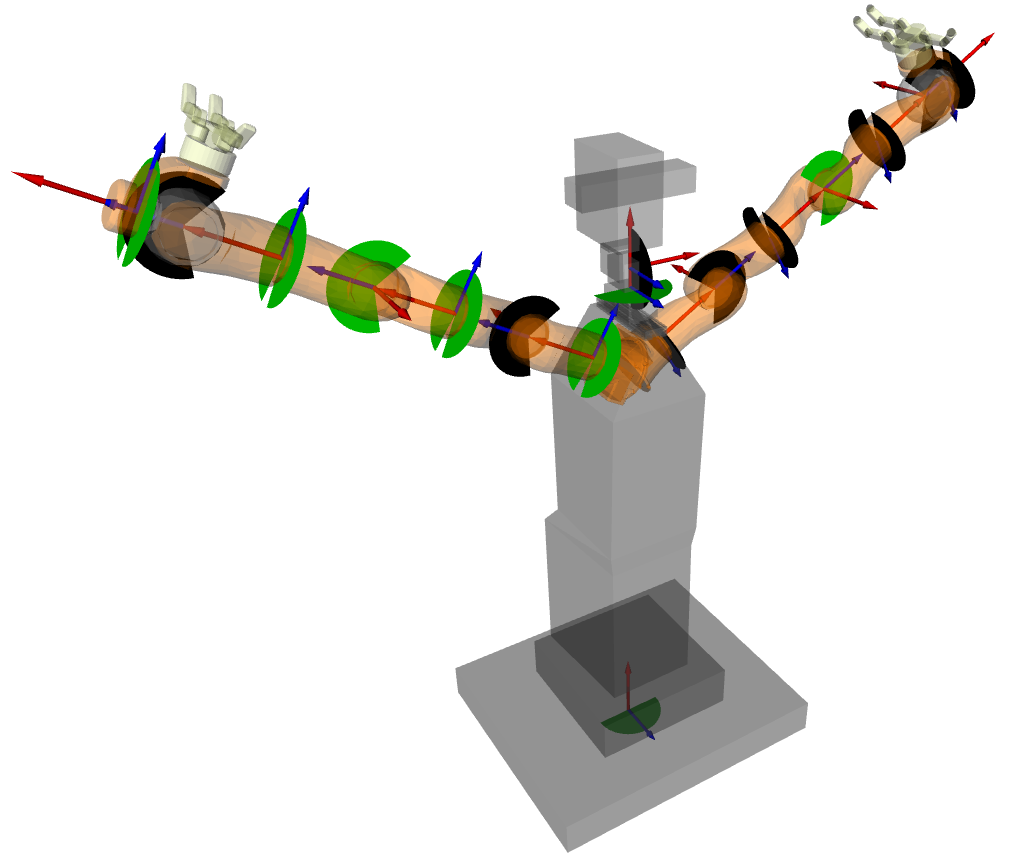
\includegraphics[width=0.65\textwidth]{obrazy/velma_joints.png}
		\caption{Robot Velma (źródło: \cite{robotVelma})}
		\label{f:robot_Velma}
	\end{figure}
	
	Tak jak w~przypadku robotów Irp-6, szeroka gama czujników pozwala na dokładne sterowanie. Zaś sterowanie impedancyjne, a~konkretnie nadawanie pożądanej sztywności stawom, daje możliwość manipulacji dynamicznych relacji robota ze środowiskiem. Dodatkowo system Velmy wywołuje wirtualne siły odpychające od siebie stawy, tak by zapobiec ich kolizji. Zarówno obniżanie sztywności w~stawach, jak i~wprowadzanie wirtualnych sił zimniejsza prawdopodobieństwo idealnego osiągnięcia zadanej pozycji.
	\section{Oprogramowanie bazowe}
	\label{s:oprogramowanie_bazowe}
	Oprogramowanie, które steruje robotami Irp-6 i~Velma opiera się na wolnodostępnych platformach. Wprowadzone modyfikacje musiały zostać stworzone w~tej samej konwencji i~technologii. 
		\subsection{ROS}
		\label{ss:ros}
		ROS (The Robot Operating System) to otwarta platforma programistyczna, która przede wszystkim definiuje sposoby komunikacji między różnymi fragmentami systemu\cite{ROS}. Poza tym implementuje narzędzia przydatne nie tylko do czystej pracy systemu, ale i~jego analizy.
		
		ROS rozdziela elementy na węzły. Założeniem systemu jest dzielenie fragmentów oprogramowania na podstawie funkcjonalności. Przykładowo analizę położenia robota można rozdzielić na kolejne węzły: zbierający informację od enkoderów/kamer, konwertujący odczyty do bardziej czytelnej formy, określający położenie na podstawie dostosowanych danych. Widać tu potrzebę przesyłu danych pomiędzy wymienionymi węzłami. Istnieją dwa podstawowe sposoby komunikacji węzłów w~systemie opartym na tej platformie:
		\begin{itemize}
			\item za pomocą tematów - jeden z~węzłów pisze informacje na temacie (publisher), inne mogą je z~niego odczytywać (subscriber);
			\item komunikacja jeden-do-jednego - jeden z~węzłów zapewnia serwis, odpowiadający na zapytanie klienta.
		\end{itemize}
		Nie jest wykluczone by węzeł był jednocześnie odbiorcą i~dostarczycielem danych. Tak samo możliwe jest by komunikacja z~węzłem przebiegała na oba sposoby. Sposoby komunikacji przedstawiono jest na rysunku~\ref{f:ros_komunikacja}.
		\begin{figure}[h]
			\centering
			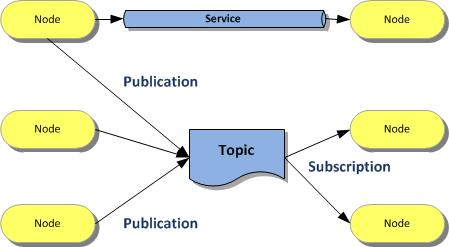
\includegraphics[width=0.8\textwidth]{obrazy/Concepts-de-base-de-ROS.jpg}
			\caption{Podstawowa komunikacja w~systemie ROS (źródło: \cite{whatROS})}
			\label{f:ros_komunikacja}
		\end{figure}
		
		
		Dodatkowo ROS wyposażony jest w bibliotekę \texttt{actionlib}. Jest to interfejs dla zadań, które można wywłaszczyć\cite{actionlibROS}. Jest to szczególnie przydatne gdy wykonanie czynności jest długotrwałe i~może zaburzyć działanie systemu. Wiadomości przekazywane pomiędzy klientem i~serwisem w~plikach deklaracji podzielone są na trzy części: gol, informacje zwrotne oraz wynik zadania. Serwer możne w~danym momencie mieć tylko jeden aktywny gol, o~którego statusie wysyłane są informacje zwrotne (np. w~każdej iteracji obliczającej ustawienia chwilowe). Biblioteka zapewnia wygody sposób na odwoływanie się do pól struktury wiadomości akcji oraz do operowania statusem celu (ustawianie go na przyjęty, odrzucony itp.). Ten sposób komunikacji jest wykorzystywany do łączenia interfejsu użytkownika sytemu IrpOS lub VelmOS z~komponentami akcji, a~przez to dedykowanymi im generatorami.
		
		\subsection{Open Robot Control Software}
		\label{ss:orocos}
		\subsection{Connman}
		\label{ss:connman}
		\subsection{Rviz}
		\label{ss:rviz}
		\subsection{Gazebo}
		\label{ss:gazebo}
	\section{System IrpOS}
	\label{s:irpos}
	\section{System VelmOS}
	\label{s:velmos}
		\subsection{rqt\_agent}
		\label{ss:rqt_agent}
		\subsection{show\_collisions}
		\label{ss:show_collisions}
		\subsection{show\_joints}
		\label{ss:show_joints}
		
	\section{Algorytmy}
	\label{s:algorytmy}